\documentclass[times, utf8, numeric, diplomski]{ferit}

\usepackage{booktabs}
\usepackage{tikz}
\usetikzlibrary{chains,arrows.meta,fit,backgrounds,shapes.geometric}
\usepackage{fancyvrb}
\usepackage{listings}
\lstset{
    language=Bash,
    tabsize=2,
    showstringspaces=false,
    columns=flexible,
    basicstyle={\footnotesize\ttfamily},
    breaklines=true,
    frame=single,
    captionpos=b,
}

% indent first paragraph
\usepackage{indentfirst}


\begin{document}
\thesisnumber{000} % TODO broj rada
\title{Sustav za kontinuirani razvoj aplikacija}

\author{Josip Šokčević}
% TODO exclude numeration
\maketitle

% TODO potrebno?
%\izvornik{}

\zahvala{}
TODO

\tableofcontents

\chapter{Uvod}
Razvoj aplikacija uvelike se promijenio s razvojem novih tehnologija, a pogotovo u zadnjem desetljeću
s razvojem oblaka (engl.~\textit{cloud}). Sve je veći broj poduzeća koji se bave razvojem aplikacija
te imaju potrebu što prije objaviti nadogradnje aplikacija. Stare metode objavljivanja aplikacija
traju dugo te vrijeme potrebno za objavu raste s rastom broja inženjera. Osim što su skupe,
podložne su i ljudskim greškama. Stoga se sve više poduzeća odlučuje za kontinuirani razvoj
aplikacija.

Korištenjem kontinuiranog razvoja aplikacija te brzog razvoja (engl.~\textit{agile development})
moguće je objavljivati nadogradnje više puta dnevno~\citep{abrahamsson2017agile} bez potrebe za
inženjerom objave (engl.~\textit{release engineer}). Takav sustav mora biti u mogućnosti otkriti
promjene na sustavu za reviziju koda, pokrenuti testove jedinice, kompajlirati aplikaciju, provesti
dodatna testiranja te poslužiti takvu aplikaciju krajnjim korisnicima.

Poduzeće Facebook objavio je članak~\citep{rossi2016continuous} o korištenju kontinuiranog razvoja
gdje nepobitno dokazuju da brzina objavljivanja novog koda ne opada sa povećanjem broj inženjera
razvojnih timova i kvaliteta koda ne opada. Broj grešaka (engl.~\textit{bugs}) u kodu linearno raste
s brojem objavljivanja koda, kao što je i očekivano. Također, neovisno o broju inženjera, u
prosjeku se pojavljuje jedna greška srednjeg prioriteta na oko 3000 pojedinačnih objava koda.
Facebook tvrdi da je jedan od razloga kontinuirano testiranje.

U drugom poglavlju opisana je jedna od infrastruktura kontinuiranog razvoja aplikacija. Opisan je
Git sustav za reviziju koda, Jenkins aplikacija za kontinuiranu integraciju programskog koda,
Docker za pohranjivanje slike aplikacije i Nginx za distribuciju i balansiranje zahtjeva korisnika.
U trećem poglavlju opisan je proces i izrada jednostavne internet aplikacije u Go programskom jeziku
zajedno s testovima jedinice i testovima funkcionalnosti. Opisana je i izrada Jenkins posla koja će
pokrenuti testove i kompajliranje te izraditi i spremiti Docker sliku. U četvrtom poglavlju opisan
je proces preuzimanje Docker te posluživanje korisnika preko Nginx programa.



\chapter{INFRASTRUKTURA KONTINUIRANOG RAZVOJA APLIKACIJA}
Za izradu sustava za kontinuiran razvoj aplikacije potrebna je infrastruktura koja to omogućuje.
Postoji velik izbor aplikacija i servisa koji se mogu koristiti u tu svrhu.  Na primjer, za
verzioniranje koda može se koristiti Git, Subversion, Mercurial, Microsoft TFS, a za kontinuiranu
integraciju programskog koda Jenkins, Hudson, TeamCity. U ovom poglavlju opisani su:
\begin{itemize}
    \item različite vrste kontrole verzije te izabrani sustav Git
    \item alat za kontinuiranu integraciju Jenkins
    \item Docker alat za upravljanje kontejnerima te razlika između kontejnera i virtualizacije
    \item Nginx web servis
    \item Go programski jezik razvijen od strane Google
    \item Cypress -- alat za \textit{end-to-end} testiranje.
\end{itemize}

\section{Git -- sustav kontrole verzija}
Sustav kontrole verzija je sustav koji sprema promjene datoteka kroz vrijeme. Najčešće se koristi za
pohranjivanje programskog koda, no takav sustav može se koristiti i za druge stvari kao što su
znanstveni radovi, dokumentacije, dizajni i slično~\citep{perez2016ten}. Prilikom izgradnje
programske podrške u pravilu je potrebno imati sustav verzija, pogotovo ako više inženjera radi na
istom projektu. Korisnik u bilo kojem trenutku može zapisati trenutno stanje mape
(\textit{engl.~directory}) u sustav. Na primjer, korisnik može zapisati kada je određena cjelina
aplikacija isprogramirana, kada je popravljena greška (\textit{engl.~bug}) ili kada su dodani novi
testovi jedinica. Korisnik može pregledati povijest u bilo kojem trenutku, vratiti mapu u prijašnje
stanje, usporediti izmjene između zapisa.  To je samo mali dio operacija koje korisnik može
odraditi.  Prema anketi Stack Overflow iz 2017, od 30.730 ispitanika, 69,2\% se izjasnilo da koristi
Git, a prati ga Subversion s 9,1\% i Microsoft TFS s 7,3\%~\citep{StackOverflow2017Survey}.
Rezultati ankete prikazni su slikom~\ref{fig:02so_survey}.

\begin{figure}[h]
    \centering
    \includegraphics[width=0.75\textwidth]{img/02/so_survey.png}
    \caption{Rezultati ankete o korištenju kontrole sustava}%
    \label{fig:02so_survey}
\end{figure}


\subsection{Vrste sustava kontrole verzija}
Prije nego što su ovakvi sustavi postali popularni i industrijski standard, korisnici su ručno
kopirali mapu ili datoteku te ju spremali kao rezervu (\textit{engl.~backup}). Takav proces podložan
je greškama te ne pruža puno funkcionalnosti. Jedno od prvih dostupnih rješenja je RCS
(\textit{engl. Revision Control System})~\citep{chacon2014pro}. RCS omogućava pohranjivanje
razlike datoteka (\textit{engl.~patch set}) između revizija. Korisnik može vratiti datoteku u
prijašnje stanje tako da sustav primjeni razliku datoteka, kao što je prikazano na
slici~\ref{fig:02rcs}.

% TODO vise teksta, povijest

\begin{figure}[h]
    \centering
    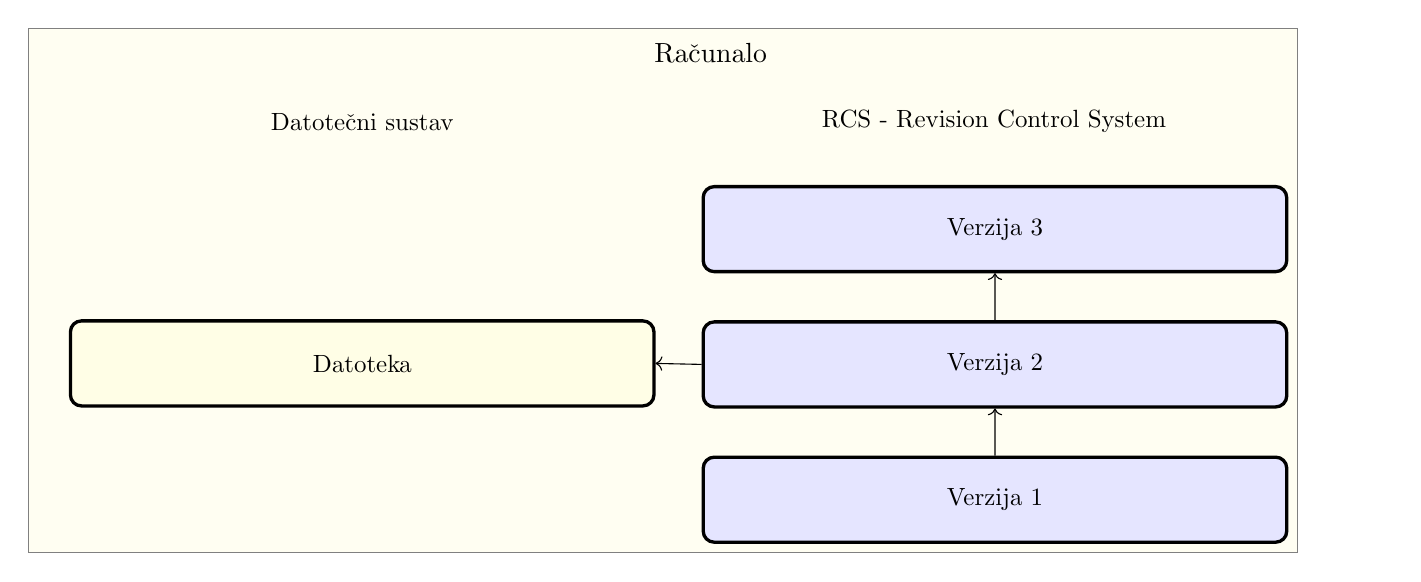
\begin{tikzpicture}[
        scale=0.7,
        start chain=1 going below,
        start chain=2 going right,
        node distance=6mm,
        text centered,
        box/.style={
            rectangle,
            rounded corners,
            draw=black,
            very thick,
            minimum height=12mm,
            fill=yellow!10
        },
        version/.style={
            fill=blue!10
        },
        l1/.style={
            text width=8cm,
            on chain=1,
            scale=0.9,
        },
        l2/.style={
            text width=8cm,
            on chain=2,
            scale=0.9,
        },
    ]

        \node [text width=8cm] (e1) {};
        \node [text width=8cm, right=of e1] (e2) {};
        % Lijevo
        \node [l1, below=of e1] (fs) {Datotečni sustav};
        \node [l1, minimum height=12mm] (empty) {};
        \node [box, l1] (file) {Datoteka};

        % Desno
        \chainin (fs); % Start right of file
        \node [l2] (rcs) {RCS - Revision Control System};
        \chainin (empty); % Start right of file
        \node [box, version, l2] (version3) {Verzija 3};
        \node [box, version, l2, continue chain=going below] (version2) {Verzija 2};
        \node [box, version, l2] (version1) {Verzija 1};

        \draw[<-] (file.east) -- (version2.west);
        \draw[<-] (version3) -- (version2);
        \draw[<-] (version2) -- (version1);

        \begin{scope}[on background layer]
            \node [draw=black!50, fill=yellow!5, fit={(e1) (version1) (fs)}] (f) {};
            \node [text width=8cm, fit={(e1) (e2)}, yshift=-2mm] (computer) {Računalo};
        \end{scope}

    \end{tikzpicture}
    \caption{Primjer lokalnog sustava kontrole verzija}%
    \label{fig:02rcs}
\end{figure}

Problemi se javljaju ukoliko je potreban rad na više računala, to jest ukoliko više inženjera
radi na projektu. Kako bi se riješio taj problem, osmišljen je centralizirani sustavi kontrole
verzija (CVCS, \textit{engl.~Centralized Version Control System}), prikazan na
slici~\ref{fig:02CVCS}. Takvi sustavi, kao što su CSV, Subversion, Perforce, imaju centralno
računalo koji sadržava sve verzije datoteka. Klijenti se spajaju na sustav kako bi kopirali datoteke
ili pohranili novu verziju.  Administratori u pravilu mogu ograničiti radnje po korisničkom računu.


\begin{figure}[h]
    \centering
    \begin{tikzpicture}[
        scale=1.0,
        node distance=4mm,
        text width=4cm,
        text centered,
        box/.style={
            rectangle,
            rounded corners,
            minimum height=12mm,
            draw=black,
            very thick,
            fill=yellow!10
        },
        version/.style={
            fill=blue!10
        },
    ]

        % Centralno racunalo
        \node [start chain=going below, text width=4.4cm] (server) {CVCS poslužitelj};
        \node [on chain, below=of computer] (db) {Baza verzija};
        \node [box, version, on chain] (version3) {Verzija 3};
        \node [box, version, on chain] (version2) {Verzija 2};
        \node [box, version, on chain] (version1) {Verzija 1};
        \node [on chain] (sp1) {};
        \draw[<-] (version3) -- (version2);
        \draw[<-] (version2) -- (version1);


        \begin{scope}[on background layer]
            \node [draw=black!50, fill=yellow!5, fit={(server) (sp1)}] (serverbox) {};
        \end{scope} \begin{scope}[on background layer]
            \node [draw=black!50, fill=white!50, fit={(db) (version1)}] (dbbox) {};
        \end{scope}

        % Klijent A
        \node [start chain=going below, right=3cm of serverbox.north east] (hidden1) {};
        \node [on chain, below=of hidden1] (client1) {Računalo A};
        \node [box, on chain, below=of client1] (file1) {Datoteka};

        \begin{scope}[on background layer]
            \node [draw=black!50, fill=yellow!5, fit={(client1) (file1)}] (client1box) {};
        \end{scope}

        % Klijent B
        \node [start chain=going below, below=of client1box] (hidden2) {};
        \node [on chain, below=of hidden2] (client2) {Računalo B};
        \node [box, on chain, below=of client2] (file2) {Datoteka};

        \begin{scope}[on background layer]
            \node [draw=black!50, fill=yellow!5, fit={(client2) (file2)}] (client2box) {};
        \end{scope}

        \draw [<-] (file1.west) -- (dbbox);
        \draw [<-] (file2.west) -- (dbbox);
    \end{tikzpicture}

    \caption{Primjer centraliziranog sustava kontrole verzija}%
    \label{fig:02CVCS}
\end{figure}

Centrali sustavi kontrole verzija imaju velike nedostatke. Kako se radi o centralom sustavu, ispadom
centralnog računala, sustav postaje nedostupan te korisnici ne mogu raditi. U slučaju gubitka
podataka na centralnim računalu, primjerice zbog kvara tvrdog diska (\textit{engl.~hard drive}),
informacije o svim revizijama su uništene, te jedini podatci koji su dostupni su oni na lokalnim
računalima korisnika. Zbog takvih nedostataka osmišljeni su distribuirani sustavi kontrole verzija.

Distribuirani sustav kontrole verzija (DVSC, \textit{engl.~Distributed Version Control System}) je
sustav u kojemu korisnik dohvaća datoteke, ali i svu povijest. Stoga, ukoliko poslužitelj postane
nedostupan, korisnik i dalje može koristiti sve funkcije takvog sustava. Isto tako, ukoliko
poslužitelj postane trajno nedostupan, korisnik može pokrenuti vlastiti poslužitelj sa podatcima
spremljenim na lokalnom računalu bez ikakvih gubitaka. Arhitektura takvog distribuiranog sustava
dana je slikom \ref{fig:02DVCS}.

\begin{figure}[h]
    \centering
    \begin{tikzpicture}[
        scale=1.0,
        node distance=3mm,
        text width=3.5cm,
        text centered,
        box/.style={
            minimum height=6mm,
            rectangle,
            rounded corners,
            draw=black,
            very thick,
            text centered,
            fill=yellow!10
        },
        title/.style={
            text width=3.7cm,
            text centered,
        },
        version/.style={
            fill=blue!10
        },
    ]

        % Posluzitelj
        \node [title, start chain=going below] (server) {DVCS poslužitelj};
        \node [on chain, below=of computer] (db) {Baza verzija};
        \node [box, version, on chain] (version3) {Verzija 3};
        \node [box, version, on chain] (version2) {Verzija 2};
        \node [box, version, on chain] (version1) {Verzija 1};
        \node [on chain] (sp1) {};
        \draw[<-] (version3) -- (version2);
        \draw[<-] (version2) -- (version1);


        \begin{scope}[on background layer]
            \node [draw=black!50, fill=yellow!5, fit={(server) (sp1)}] (serverbox) {};
        \end{scope}
        \begin{scope}[on background layer]
            \node [draw=black!50, fill=white!50, fit={(db) (version1)}] (dbbox) {};
        \end{scope}

        % Klijent A
        \node [right=3cm of serverbox.north east] (hidden1) {};
        \node [above=39mm of hidden1] (hidden11) {};
        \node [title, on chain, below=of hidden11] (client1) {Računalo A};
        \node [box, on chain, below=of client1] (file1) {Datoteka};

        \node [on chain] (c1db) {Baza verzija};
        \node [box, version, on chain] (c1version3) {Verzija 3};
        \node [box, version, on chain] (c1version2) {Verzija 2};
        \node [box, version, on chain] (c1version1) {Verzija 1};
        \node [on chain] (c1sp1) {};
        \draw[<-] (c1version3) -- (c1version2);
        \draw[<-] (c1version2) -- (c1version1);

        \begin{scope}[on background layer]
            \node [draw=black!50, fill=yellow!5, fit={(client1) (c1sp1)}] (client1box) {};
        \end{scope}
        \begin{scope}[on background layer]
            \node [draw=black!50, fill=white!50, fit={(c1db) (c1version1)}] (c1dbbox) {};
        \end{scope}
        \draw[->] (c1dbbox) -- (file1);

        % Klijent B
        \node [start chain=going below, below=of client1box] (hidden2) {};
        \node [title, on chain, below=of hidden2] (client2) {Računalo B};
        \node [box, on chain, below=of client2] (file2) {Datoteka};

        \node [on chain] (c2db) {Baza verzija};
        \node [box, version, on chain] (c2version3) {Verzija 3};
        \node [box, version, on chain] (c2version2) {Verzija 2};
        \node [box, version, on chain] (c2version1) {Verzija 1};
        \node [on chain] (c2sp1) {};
        \draw[<-] (c2version3) -- (c2version2);
        \draw[<-] (c2version2) -- (c2version1);

        \begin{scope}[on background layer]
            \node [draw=black!50, fill=yellow!5, fit={(client2) (c2sp1)}] (client2box) {};
        \end{scope}
        \begin{scope}[on background layer]
            \node [draw=black!50, fill=white!50, fit={(c2db) (c2version1)}] (c2dbbox) {};
        \end{scope}

        \draw [<->] (client1box.west) -- (serverbox);
        \draw [<->] (client2box.west) -- (serverbox);
        \draw [<->] (client2box.north) -- (client1box.south);
        \draw[->] (c2dbbox) -- (file2);
    \end{tikzpicture}

    \caption{Primjer distribuiranog sustava kontrole verzija}%
    \label{fig:02DVCS}
\end{figure}

\subsection{Osnove Git-a}
Git je distribuirani sustav otvorenog koda za kontrolu verzije. Za razliku od većine drugih VSC, Git
sprema cijele datoteke koje su promijenjene od zadnje verzije. Na primjer, ako korisnik promjeni
datoteku tako što doda novu liniju koda, klasični VSC sustavi će spremiti informaciju o toj razlici,
dok će Git spremiti cijelu datoteku. Spremanje cijele datoteke zauzima diskovni prostor, no s druge
strane omogućuje brže operacije pregledavanja povijesti te sadržaja datoteka u bilo kojem trenutku.
Zbog svoje distribuirane naravi Git je dostupan korisnicima i kada računalo nije mrežno povezano.
Većina operacija, kao što su \texttt{git-commit}, \texttt{git-merge}, \texttt{git-checkout},
\texttt{git-log}, izvršavaju se na lokalnom računalu. Kada je računalo ponovno povezano na mreži
korisnik može odabrati dohvaćanje novih datoteka ili pak slanje izmjena.

Git ima tri moguća stanja datoteka: predan (\textit{engl.~committed}), izmijenjen
(\textit{engl.~modified}) i priređen (\textit{engl.~staged}). Predane datoteke su one datoteke koje
su spremljene u lokalnu bazu, odnosno bazu na lokalnom računalu. Izmijenjene datoteke su one
datoteke koje su izmijenjene na lokalnom računalu, no nisu spremljene u lokalnoj Git bazi podataka.
Priređene datoteke su izmijenjene datoteke koje se dodaju u sljedećem unosu u Git bazu.

Jedna od značajki Git-a su grane (\textit{engl.~branch}) koje omogućuju razvoj novih funkcija
programa van glavne grane. Prilikom razvoja, manji dijelovi koda se često spremaju (\texttt{tzv.
git-commit}) i povremeno šalju na server (tzv.~\texttt{git-push}). Kada je nova funkcija
isprogramirana i testirana, takva grana se spaja (tzv.~\texttt{git-merge}) na glavnu granu. U
slučaju sukoba datoteka (\textit{engl.~conflict}), korisnik je obaviješten te mora ručno riješiti
takav sukob i ponovno testirati aplikaciju.

Korištenje Git uvelike je pojednostavljeno ukoliko se korisnik odluči koristiti servis kao što je
GitHub, Gitlab ili Bitbucket. Takvi servisi omogućuju jednostavno stvaranje Git baze te operacije
spajanja \texttt{git-merge}. Također, većina integriranih sustava za razvoj (IDE,
\textit{engl.~Integrated Development Environment}) podržava Git operacije, tako da korisnik ne mora
koristiti komandnu liniju.

\subsection{Korištenje Git-a i GitHub} Git operacije se često izvode preko komandne linije.
Kreiranje novog Git projekta obavlja se preko komande \texttt{git-init}. Git-init stvara praznu Git
bazu podataka. Korisnik nakon toga može prirediti datoteke koje će se spremiti u bazu preko
operacije \texttt{git-add}. Kada je sve spremno za trajno spremanje u Git bazu, pokreće se operacija
\texttt{git-commit} koja predaje datoteke u lokalnu Git bazu. Primjer stvaranja Git projekta te
spremanja prikazan je programskim kodom~\ref{02init}.

\lstset{caption={Kreiranje Git projekta i prvo predavanje}, label=02init}
\begin{lstlisting}[float=h]
git init
git add main.go // Pretpostavka da main.go postoji unutar direktorija
git add LICENSE // Pretpostavka da LICENSE postoji unutar direktorija
git commit -m "Prvi commit"
\end{lstlisting}

Takva baza spremljena je na lokalnom računalu te je samim time nedostupna drugim računalima. Kako bi
takva baza postala dostupna drugim računalima, potrebno je poslati bazu na Git poslužitelj. Jedan od
najpopularnijih servisa koji pruža Git poslužitelj kao uslugu je GitHub.  U travnju 2017. godine
GitHub je objavio da je registrirano skoro 20 milijuna korisnika i 57 milijuna Git
projekata~\citep{github2017}. Korisnik se mora registrirati na github.com kako bi mogao koristiti
usluge. Nakon uspješne registracije, Git projekt se može kreirati kao što je prikazano na
slici~\ref{fig:02hgreg}.

\begin{figure}[h]
    \centering
    \includegraphics[width=\linewidth]{img/02/gh.png}
    \caption{Registracija Git projekta na github.com}%
    \label{fig:02hgreg}
\end{figure}

Kada je napravljen projekt na GitHub-u, u lokalnu bazu registrira se udaljen Git poslužitelj pomoću
\texttt{git-remote} operacije te se lokalna baza može poslati na udaljeno računalo pomoću operacije
\texttt{git-push}. Važno je zapamtiti da operacija \texttt{git-commit} ne šalje izmjene na udaljeno
računalo, nego isključivo \texttt{git-push}.  Operacija \texttt{git-push} šalje samo razliku između
lokalnih predanih datoteka te udaljenih datoteka.  Primjer dodavanja udaljenog servera i slanje
izmjena dan je programskim kodom~\ref{02remote}

\lstset{caption={Dodavanje poslužitelja i slanje izmjena}, label=02remote}
\begin{lstlisting}[float=h]
git remote add origin git@github.com:sokac/diplomski-go.git
git push -u origin master
\end{lstlisting}

\subsection{Git grane}
Većina VSC sustava podržava neku vrstu grananja. Grananje omogućava korisniku da izađe iz glavne
grane razvoja, često nazvanu \textit{master}, te nastavi razvoj u potpuno drugoj grani. Korisnik u
bilo kojem trenutku može izabrati u kojoj grani želi biti. Također, korisnik može spojiti dvije
grane u bilo kojem trenutku.  Git ima prednost nad drugim VSC sustavima jer su stvaranje i
mijenjanje grana izuzetno brze operacije. Samim time, Git potiče na često korištenje grana. Nova
grana stvara se operacijom \texttt{git-branch} te ima iste datoteke kao i grana prije nego što je
operacija stvaranja grane bila pozvana. Operacija \texttt{git-checkout} koristi se za prebacivanje u
drugu granu. Trenutna grana zapisana je u specijalnoj referenci koja se zove \textit{HEAD}. Na
slici~\ref{fig:02gitexample} prikazan je Git projekt s dvije grane, \textit{master} i
\textit{development}, gdje grana \textit{development} sadrži više predanih izmjena. Prilikom
pokretanja \texttt{git checkout master}, \textit{HEAD} pokazivač se pomiče na \textit{master} granu
te se datoteke mijenjaju na sadržaj \textit{master} grane, kao što je prikazano na
slici~\ref{fig:02gitexample2}. Ukoliko korisnik preda izmjene unutar grane \textit{master}, tada
dolazi do razdvajanja grana, jer grana \textit{master} ima datoteke koje ne postoje u povijesti
grane \textit{development} i obrnuto. Git operacija \texttt{git-merge} omogućava spajanje grana i u
takvom slučaju. Osim standardnih operacija, Github servis nudi uslugu pregleda koda (\textit{engl.
code review}). Inženjeri mogu međusobno pregledavati kod prije nego što se spoji s glavnom granom.
Također je moguće koristiti i integracijske testove kako bi se osiguralo ispravno funkcioniranje
novog koda.

\begin{figure}[h]
    \centering
    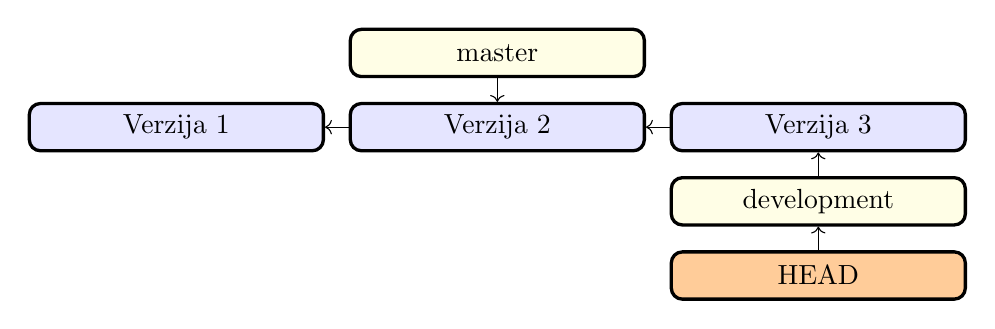
\begin{tikzpicture}[
        scale=1.0,
        node distance=3mm,
        text width=3.5cm,
        text centered,
        box/.style={
            minimum height=6mm,
            rectangle,
            rounded corners,
            draw=black,
            very thick,
            text centered,
            fill=yellow!10
        },
        head/.style={
            fill=orange!40
        },
        version/.style={
            fill=blue!10
        },
    ]
        \node [box, version] (c1version1) {Verzija 1};
        \node [box, version, right=of c1version1] (c1version2) {Verzija 2};
        \node [box, version, right=of c1version2] (c1version3) {Verzija 3};
        \node [box, above=of c1version2] (master) {master};
        \node [box, below=of c1version3] (development) {development};
        \node [box, head, below=of development] (head) {HEAD};
        \draw [<-] (c1version1) -- (c1version2);
        \draw [<-] (c1version2) -- (c1version3);
        \draw [->] (development) -- (c1version3);
        \draw [->] (master) -- (c1version2);
        \draw [->] (head) -- (development);

    \end{tikzpicture}

    \caption{Primjer Git grana}%
    \label{fig:02gitexample}
\end{figure}

\begin{figure}[h]
    \centering
    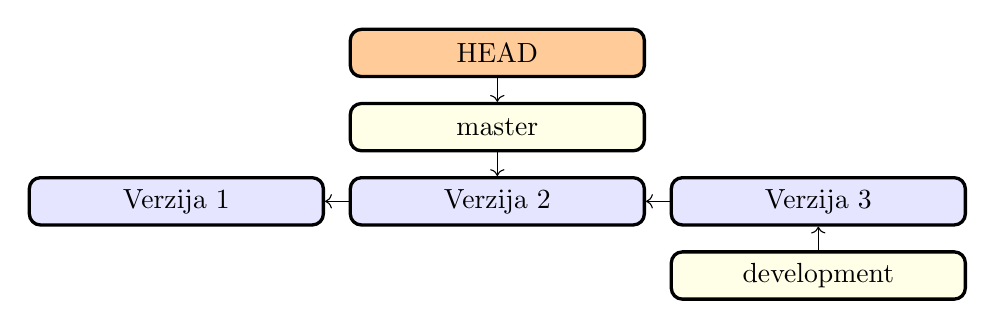
\begin{tikzpicture}[
        scale=1.0,
        node distance=3mm,
        text width=3.5cm,
        text centered,
        box/.style={
            minimum height=6mm,
            rectangle,
            rounded corners,
            draw=black,
            very thick,
            text centered,
            fill=yellow!10
        },
        head/.style={
            fill=orange!40
        },
        version/.style={
            fill=blue!10
        },
    ]
        \node [box, version] (c1version1) {Verzija 1};
        \node [box, version, right=of c1version1] (c1version2) {Verzija 2};
        \node [box, version, right=of c1version2] (c1version3) {Verzija 3};
        \node [box, above=of c1version2] (master) {master};
        \node [box, below=of c1version3] (development) {development};
        \node [box, head, above=of master] (head) {HEAD};
        \draw [<-] (c1version1) -- (c1version2);
        \draw [<-] (c1version2) -- (c1version3);
        \draw [->] (development) -- (c1version3);
        \draw [->] (master) -- (c1version2);
        \draw [->] (head) -- (master);

    \end{tikzpicture}

    \caption{Primjer pomicanja Git grane}%
    \label{fig:02gitexample2}
\end{figure}

\section{Jenkins}
Timovi koji koriste stare metode, kao što su Grantt dijagrame i model vodopada (\textit{engl.
waterfall model}), moraju odvojiti poveći dio vremena za fazu integracije. U toj fazi razvoja
računalne podrške inženjeri i timovi spajaju dijelove koda na kojima su radili mjesecima. Prilikom
spajanja, često dolazi do sukoba datoteka i programskih sučelja koji inženjeri ručno moraju
riješiti. Taj proces zna potrajati tjednima jer je potrebno riješiti sukobe i ponovno testirati
program. U takvom je sustavu faza integracija izuzetno stresna za inženjere i voditelje timove. Ta
faza je često uzrok odgađanja objavljive nove verzije, a samim time i gubitak povjerenja krajnjih
korisnika. Iz tih je razloga nastala potreba za kontinuiranom integracijom.

Kontinuirana integracija (CI, \textit{engl.~Continuous Integration}) je način razvoja aplikacije
gdje se radne verzije programa spajaju s glavnom verzijom barem jednom
dnevno~\citep{fowler2006continuous}. Ekstremnija verzija takvog načina razvoja nazvana je ekstremno
programiranje (XP, \textit{engl.~Extreme Programming}), gdje se radna verzija spaja u glavnu verziju
barem jednom u dva do tri sata~\citep{beck1999embracing}, kako je prikazano na slici~\ref{fig:02xp}.
Kako bi to bilo moguće potrebna je dobra infrastruktura koja omogućava brzo otkrivanje grešaka
prilikom razvoja. Ona također pomaže prilikom dijagnostike te omogućava brzu izgradnju aplikacije.
Svaki bi profesionalni razvojni tim trebao koristiti takav sustav kako bi bio što učinkovitiji i
konkurentniji.

\begin{figure}[h]
    \centering
    \includegraphics[width=0.6\textwidth]{img/02/xp.png}
    \caption{Extremno programiranje}
    \label{fig:02xp}
\end{figure}

Pojednostavljeno, sustav kontinuirane integracije nadgleda sve promjene nad sustavom kontrole
verzija. Kada je promjena očitana, sustav pokreće proces testiranja jedinica i izgradnje aplikacije
(\textit{engl. compile}). U slučaju greške, sustav obavještava inženjera o pogrešci kako bi se mogla
ispraviti što prije. Osim toga, sustav mora biti u mogućnosti proizvesti izvješća o kvaliteti koda,
kao što je pokrivenost testiranja jedinice, razne statistike poput vrijeme izgradnje, učestalost
grešaka. Ako je sustav kontinuirane integracije pouzdan, može se automatizirati i sustav
objavljivanja aplikacija. Ukoliko se takva aplikacija automatski objavljuje i dostavlja krajnjim
korisnicima, radi se o sustavu za kontinuirani razvoj i objavu aplikacija (\textit{engl.~Continuous
Deployment}). Kod takvog sustava iznimno je bitno da je proces nadogradnje aplikacije jednostavan, a
poželjno i skriven od krajnjeg korisnika. Stoga se najčešće primjenjuje na mrežnim aplikacijama kao
što su internet aplikacije i stranice.

% TODO više o povijesti
Jenkins, izvorno nazvan Hudson, je alat za kontinuiranu integraciju otvorenog koda napisan u
programskom jeziku Java. Postao je iznimno popularan zbog jednostavnosti korištenja, jednostavnog
grafičkog sučelja, mogućnosti proširenja preko dodataka (\textit{engl. plugins}) te mnogih drugih
značajki. Primjer početne stranice Jenkinsa prikazan je na slici~\ref{fig:02jenkins_home}.

\begin{figure}[h]
    \centering
    \includegraphics[width=\textwidth]{img/02/jenkins_home.png}
    \caption{Jenkins početna stranica}%
    \label{fig:02jenkins_home}
\end{figure}

Jenkins alat može se postepeno uvesti u tvrtkama koji nemaju nikakav sustav kontinuirane
integracije~\citep{smart2011jenkins}. Prvo je potrebno uvesti sustav koji će na dnevnoj bazi
izgrađivati aplikaciju. Druga faza je uvođenje automatskog testiranja prije izgrađivanja aplikacije,
također na dnevnoj razini. Sljedeća faza je uvođenje metrika za kvalitetu koda (pokrivenosti
jedinica, brzina testova i izgradnje) te automatska izgradnja dokumentacije. Četvrta faza je dodatno
testiranje, poput testiranja funkcionalnosti, a ona se odvija nakon što je aplikacija izgrađena.
Peta faza je automatsko objavljivanje aplikacije koja je prošla dodatno testiranje. Takvu
aplikaciju mogu koristiti i osobe koje nisu inženjeri, kao što su timovi za testiranje kvalitete.
Zadnja faza sustava je kontinuirano objavljivanje aplikacije krajnjim korisnicima. Jenkins se
sastoji od:
\begin{itemize}
    \item poslova (\textit{engl. Jobs})
    \item građe (\textit{engl. build})
    \item parametara
    \item linije (\textit{engl. Pipeline})
    \item dodataka (\textit{engl. plugins}).
\end{itemize}

\subsection{Jenkins arhitektura}
Jenkins posao je skup pravila prema kojemu se izgrađuje aplikacija. Sastoji se od naziva posla,
opisa, definiranih parametara potrebnih za pokretanje izgradnje aplikacije, instrukcija za
izgradnju aplikacije te listu akcija nakon što je posao završen~\citep{pathania2016learning}.
Jenkins posao ne ovisi o programskom jeziku aplikacije koja se izgrađuje niti o VCS. Posao se može
programirati, ali i izgraditi koristeći grafičko web sučelje. Primjer izgradnje posla preko web
sučelja prikazan je slikom~\ref{fig:02jenkinsjob}.

\begin{figure}[h]
    \centering
    \includegraphics[width=0.8\textwidth]{img/02/jenkins_job.png}
    \caption{Izgradnja Jenkins posla preko grafičkog sučelja}%
    \label{fig:02jenkinsjob}
\end{figure}

Jenkins parametri često se koriste za Jenkins poslove. Jenkins podržava velik broj tipova
parametara, kao što su riječi, brojevi, izbornici, jedno-bitni podatci (da/ne odgovor). Parametri se
mogu automatski predavati poslu ili ručno. Primjer automatskog predavanja parametara je kada jedan
Jenkins posao pokreće drugi te predaje informacije o prethodnom izvršavanju. Primjer ručnog
predavanja parametara je kada korisnik odabere verziju koju želi pokrenuti. Većina Jenkins poslova
sadrže barem jednu Jenkins građu. Jenkins građa je jedinica posla koja se izvršava kada se Jenkins
posao izvršava. Može biti jednostavna Linux Bash ili Windows batch naredba, a preko dodataka može
izvršavati i kompleksne stvari kao što su Python skripte, Groovy, preuzimanje Android dodataka, itd.
Primjer Jenkins posla s jednom građom prikazan je slikom~\ref{fig:02jenkins_pipeline}. Jedan
Jenkins posao može imati više Jenkins građi. Jenkins linija omogućava umrežavanje više Jenkins
poslova. Linija može pokrenuti Jenkins poslove sekvencijalno ili paralelno te može sadržavati
logiku. Na primjer, Jenkins linija može odlučiti da se linija prekida ukoliko jedan od paralelnih
poslova bude neuspješan. Pomoću akcija nakon građe (\textit{engl. Post-Build}) korisnici mogu biti
obaviješteni o rezultatima građe. Jedna od velikih prednosti Jenkins alata jest upravo u dodatcima.
Dodatci mogu mijenjati vizualno web sučelje, mijenjati način povezivanja Jenkins gazde s Jenkins
slugom, dodati podršku za nove programske jezike i VSC. U službenom Jenkins repositoriju
registrirano je preko tisuću različitih dodataka~\citep{JenkisPlugins}.

\begin{figure}[h]
    \centering
    \includegraphics[width=\textwidth]{img/02/jenkins_pipeline.png}
    \caption{Jenkins građa pomoću Pipeline skripte}%
    \label{fig:02jenkins_pipeline}
\end{figure}

\section{Docker}
Docker je projekt otvorenog koda napisan u Go programskom jeziku koji pojednostavljuje objavljivanje
programa tako što koristi programske kontejnere (\textit{engl. Software Containers}). Unutar
\texttt{Unix} okruženja često se koristio izraz zatvor (\textit{engl. jail}) prilikom izmjene
okoline radi sigurnosne izolacije procesa i resursa. S izlaskom Solaris Linux 2005.  godine i
izmjene u sustavu izolacije počinje se upotrebljavati izraz kontejneri~\citep{nickoloff2016docker}.
Po zadanoj vrijednosti (\textit{engl. default value}) kontejneri nemaju pristup nikakvih resursima,
što uključuje diskovne, memorijske, sabirničke te mrežne resurse. Korisnik može dozvoliti određene
resurse ukoliko je to potrebno. Iako kontejneri postoje već dugi niz godina, korištenje istih nije
bilo jednostavno sve do pojave Docker projekta.

Docker je konceptno sličan virtualizaciji, kao što je VMWare i VirtualBox. No, za razliku od
virtualizacije, prednost Dockera je u tome što je brži i koristi manje
resursa~\citep{leszko2017continuous}. Docker koristi Linux jezgru glavnog računala. Na
slici~\ref{fig:02vm} prikazana je arhitektura kod tipične virtualizacije, dok je na
slici~\ref{fig:02docker} prikazana Docker arhitektura.

\begin{figure}[h]
    \centering
    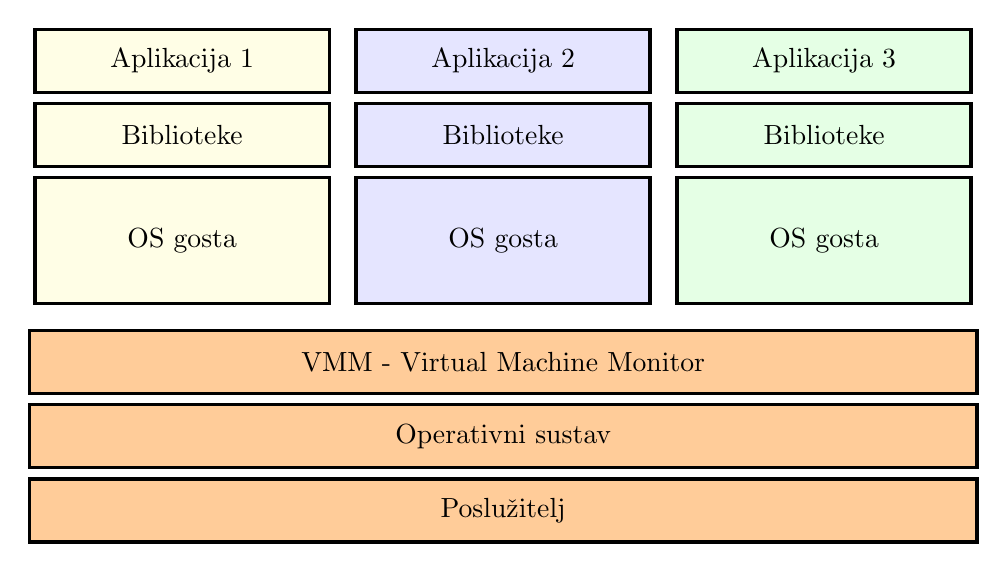
\begin{tikzpicture}[
        scale=1.0,
        node distance=1mm,
        text width=3.5cm,
        text centered,
        box/.style={
            minimum height=8mm,
            rectangle,
            draw=black,
            very thick,
            text centered,
        },
        box1/.style={
            fill=yellow!10,
        },
        box2/.style={
            fill=blue!10,
        },
        box3/.style={
            fill=green!10,
        },
        os/.style={
            minimum height=16mm,
        },
        big/.style={
            fill=orange!40,
            text width = 11.8cm,
        },
    ]
        \node [box, big] (server) {Poslužitelj};
        \node [box, big, above=of server] (os) {Operativni sustav};
        \node [box, big, above=of os] (vmm) {VMM - Virtual Machine Monitor};

        \node [box, box2, os, above=3mm of vmm] (g2os) {OS gosta};
        \node [box, box2, above=of g2os] (g2bib) {Biblioteke};
        \node [box, box2, above=of g2bib] (g2app) {Aplikacija 2};

        \node [box, box1, os, left=3mm of g2os] (g1os) {OS gosta};
        \node [box, box1, above=of g1os] (g1bib) {Biblioteke};
        \node [box, box1, above=of g1bib] (g1app) {Aplikacija 1};

        \node [box, box3, os, right=3mm of g2os] (g3os) {OS gosta};
        \node [box, box3, above=of g3os] (g3bib) {Biblioteke};
        \node [box, box3, above=of g3bib] (g3app) {Aplikacija 3};
    \end{tikzpicture}

    \caption{Arhitektura virtualizacije}%
    \label{fig:02vm}
\end{figure}

\begin{figure}[h]
    \centering
    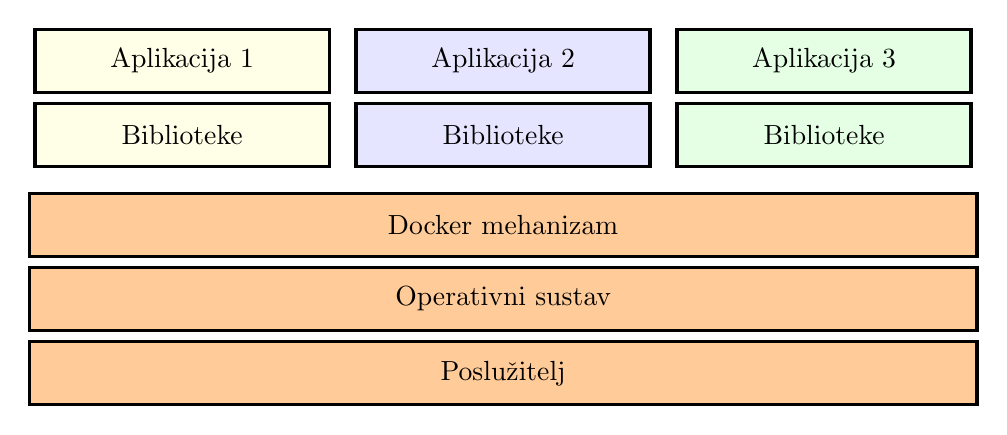
\begin{tikzpicture}[
        scale=1.0,
        node distance=1mm,
        text width=3.5cm,
        text centered,
        box/.style={
            minimum height=8mm,
            rectangle,
            draw=black,
            very thick,
            text centered,
        },
        box1/.style={
            fill=yellow!10,
        },
        box2/.style={
            fill=blue!10,
        },
        box3/.style={
            fill=green!10,
        },
        big/.style={
            fill=orange!40,
            text width = 11.8cm,
        },
    ]
        \node [box, big] (server) {Poslužitelj};
        \node [box, big, above=of server] (os) {Operativni sustav};
        \node [box, big, above=of os] (docker) {Docker mehanizam};

        \node [box, box2, above=3mm of docker] (g2bib) {Biblioteke};
        \node [box, box2, above=of g2bib] (g2app) {Aplikacija 2};

        \node [box, box1, left=3mm of g2bib] (g1bib) {Biblioteke};
        \node [box, box1, above=of g1bib] (g1app) {Aplikacija 1};

        \node [box, box3, right=3mm of g2bib] (g3bib) {Biblioteke};
        \node [box, box3, above=of g3bib] (g3app) {Aplikacija 3};
    \end{tikzpicture}

    \caption{Docker arhitektura}%
    \label{fig:02docker}
\end{figure}

Docker slika (\textit{engl. Docker Image}) je preslika datotečnog sustava koja se sastoji od niza
Docker slojeva (\textit{engl. Docker layers}). Slojevi predstavljaju promjene u datotečnom sustavu
naspram prijašnjeg sloja. Docker kontejner koristi Docker sliku te pokreće određenu aplikaciju koja
se već nalazi unutar Docker slike. Promjene unutar Docker kontejnera, kao što je zapis novih
datoteka, ne mijenjaju Docker sliku korištenu za pokretanje tog kontejnera. Kada se Docker
kontejner zaustavi i obriše, svi podatci su također obrisani. Docker slika pakira program unutar
cjelokupnog datotečnog sustava koji ima sve potrebne komponente kako bi se takav program mogao
izvoditi - od dinamičkih modula, biblioteka, sve do programskog sučelja operativnoga sustava. Stoga
Docker garantira da će izvršavanje takvog sustava bit uvijek jednako, neovisno o računalo na kojemu
se izvodi. Slike mogu se spremiti u Docker repositorij koji može biti privatni ili javni. Jedan od
najčešće korištenih je službeni repositorij kompanije koja stoji iza Docker-a - Docker, Inc, a koji
se nalazi na Web stranici \textit{https://hub.docker.com}. Kako bi se Docker slika pokrenula,
potrebno je imati pokrenuti Docker servis (~\textit{engl. daemon}) te imati Docker komandni
program. Korisnik zatim pokreće Docker komandni program koji potom komunicira s Docker servisom.
Docker servis može biti pokrenut na lokalnom ili udaljenom računalu.

\subsection{Docker komandni program}
Izgradnja Docker slike pokreće se pomoću naredbe \texttt{docker~build}. Ta naredba učitava datoteku
\textit{Dockerfile} u zadanom direktoriju te šalje naredbu Docker servisu. \textit{Dockerfile} je
tekstualni dokument koji sadrži instalacijske instrukcije potrebne za izgradnju Docker
slike~\citep{kacamarga2015lightweight}. Na primjeru danim kodom~\ref{02dockerfile} prikazana je
instalacija Jenkins alata.

\lstset{caption={Jenkins Dockerfile}, label=02dockerfile}
\begin{lstlisting}[float=h]
FROM openjdk:8-jdk-alpine

RUN addgroup -g 1000 jenkins
RUN adduser -u 1000 -G jenkins jenkins

RUN curl -fsSL \
    https://repo.jenkins-ci.org/public/org/jenkins-ci/main/jenkins-war/2.117/jenkins-war-2.117.war \
    -o /usr/share/jenkins/jenkins.war

USER jenkins

ENTRYPOINT ["java", "-jar", "/usr/share/jenkins/jenkins.war"]
\end{lstlisting}

U danom primjeru korištene su četiri naredbe. Naredbna \texttt{FROM} definira Docker sliku na kojoj
će se nova slika temeljiti. Na primjeru ona se temelji na \textit{openjdk} slici pod oznakom
\textit{8-jdk-alpine}. Naredba \texttt{RUN} pokreće program koji je definiran iza te naredbne. U
danom primjeru pokrenuta je komanda \texttt{addgroup} koja stvara Jenkins groupu, naredba
\texttt{adduser} koja stvara Jenkins korisnika te \texttt{curl} koja dohvaća Jenkins alat s
udaljenog računala.  Naredba \texttt{USER} definira pod kojim korisnikom se pokreće Docker
kontejner. U danom primjeru riječ je o  korisniku \textit{jenkins}. Zadnja korištena naredba
\texttt{ENTRYPOINT} definira koji će se program pokrenuti unutar Docker kontejnera, a u danom
primjer je \texttt{java -jar /usr/share/jenkins/jenkins.war}.

Nakon što je Docker slika izgrađena, korisnik može pokrenuti Docker kontejner koristeći
novoizgrađenu sliku pomoću naredbe \texttt{docker~run}. Prilikom pokretanja takve naredbe, korisnik
može podesiti mrežne postavke, montirati direktorije, ograničiti procesorske, diskovne i memorijske
resurse, izmjeniti sigurnosne postavke te mnoge druge parametre.

Jedan od najčešće korištenih parametera za mrežne aplikacije jeste parametar \texttt{-p}. Prilikom
pokretanja Docker kontejnera, mreža je podešena u tzv.~\textit{mostovnom} načinu rada te samim time
pristup Docker kontejneru nije moguć u lokalnoj mreži. Parametar \texttt{-p} naređuje Docker sustavu
da objavi mrežni port unutar kontejnera na glavnom računalu. Na primjer, parametar \texttt{-p
8080:80} preusmjerava mrežne zahtjeve porta 8080 na glavnom računalu prema mrežnom portu 80 unutar
Docker kontejnera. Promjena mrežnog načina rada moguća je preko parametra \texttt{-{}-network}.

Svi podatci koji su spremljeni unutar kontejnera su trajno obrisani pri brisanju istoga. Montiranje
direktorija koristi se ukoliko aplikacija sprema bitne podatke na tvrdi disk te nije dopušteno
brisanje. Svi zapisi na montirani direktorij spremaju se na tvrdi disk glavnog računala, a Docker
kontejner ima puni pristup njima. Na primjer, parametar \texttt{-v /glavno/racunalo:/data} montira
direktorij glavnog računala pod nazivom \texttt{/glavno/racunalo} na direktorij Docker kontejnera
pod nazivom \texttt{/data}. Kada Docker kontejner napravi izmjenu unutar \texttt{/data} direktorija,
takva izmjena bit će automatski dostupna unutar glavnog računala pod direktorijem
\texttt{/glavno/racunalo}.

Zaustavljanje pokrenutog Docker kontejnera izvršava se pomoću naredbe \texttt{docker~stop} koji
prihvaća listu Docker kontejnera koje se želi ugasiti. Docker servis prvo šalje \texttt{SIGTERM}
signal aplikaciji. Ukoliko aplikacija nije zaustavljane unutar perioda milosti (\textit{engl. grace
period}), tada Docker šalje \texttt{SIGKILL} signal.  Zaustavljeni Docker kontejner može se ponovno
pokrenuti naredbom \texttt{docker~start}. Naredbom \texttt{docker~rm} briše se kontejner zajedno sa
svim podatcima spremljenima unutar kontejnera.

\subsection{Docker servis}
Docker servis sadrži algoritame za izgradnju slika, pokretanje kontejnera i njihovo upravljanje.
Docker komandna linija omogućava korisniku jednostavnu komunikaciju s Docker servisom, koja se
odvija preko RESTful API koji je dokumentiran i otvoren. Docker također podržava SDK (\textit{engl.
Software Development Kit}) za Go i Python programski jezik.

Postoje tri grupe izolacije pristupa pojedinih Docker kontejnera:

\begin{itemize}
        \item podatkovni pristup
        \item mrežni pristup
        \item resursni pristup
\end{itemize}

Aplikacije koje spremaju podatke, poput baze podataka, moraju trajno spremiti dokumente na tvrdi
disk. Ukoliko je Docker kontejner s takvom aplikacijom pokrenut bez podatkovnog pristupa, svi
dokumenti spremaju se unutar radnog sloja Docker kontejnera. Docker slojevi spremljeni su na tvrdi
disk, a njihov format može izabrati sam korisnik. Neke od opcija su \texttt{aufs},
\texttt{devicemapper}, \texttt{overlay2}, \texttt{zfs}. No, ukoliko korisnik želi promjeniti Docker
sliku zbog nadogradnje ili promjene postavke, potrebno je pokrenuti novi kontejner. Prebacivanje
podataka s jednog kontejnera na drugi nije trivijalno, stoga je preporuka korištenje Docker volumena
(\textit{engl. Docker Volume}). Docker volumen može se montirati na bilo koji direktorij, a na
slici~\ref{fig:02docker_volume} prikazana je montaža na \texttt{/data} direktorij.

\begin{figure}[h]
    \centering
    \includegraphics[width=\textwidth]{img/02/docker_volume.png}
    \caption{Docker volumen montiran na \textit{/data}}%
    \label{fig:02docker_volume}
\end{figure}

Postoje dvije vrste volumena: volumen vezne montaže (\textit{engl. Bind mount volume}) i Docker
upravljani volumen (\textit{engl. Docker-managed volume}). Oba tipa volumena zahtjevaju montažni
direktorij (\textit{engl.~mount point}) unutar Docker kontejnera, no razlika je u tome gdje se
podatci spremaju. Volumen vezne montaže je vrsta volumena koja je direktno povezana s direktorijem
na glavnom računalu. Takvi volumeni korisni su ako glavno računalo mora imati direktan pristup
podatcima, u slučaju ako korisnik koristi Docker kontejner za pokretanje web poslužitelja i želi
biti u mogućnosti izmjeniti HTML datoteke. Montaža se odvija prilikom pokretanja Docker kontejnera s
parametrom \texttt{-v /glavno/racunalo:/kontejner}. Za razliku od volumena vezne montaže, Docker
upravljani volumeni su stvoreni i upravljani preko Docker servisa. Također se koristi paramtar
\texttt{-v}, no, za razliku od vezne montaže, zadaje se samo lokacija na kontejneru. Na primjer, za
naredbeni parametar \texttt{-v /direktorij} Docker će stvoriti volumen te će ga montirati na
kontejner unutar \texttt{/direktorij}. Docker volumeni mogu se monitrati samo za čitanje, te isti
mogu biti montirani na više Docker kontejnera u istom trenutku.

Aplikacije koje imaju potrebu za mrežnim pristupom, poput web servisa ili servisa elektroničke
pošte, mogu se pokrenuti unutar Docker kontejnera. Najčešće se koristi virtualna mreža po
kontejneru~(\textit{engl.~single-host virtual network}), prikazana na
slici~\ref{fig:02docker_networking}. To omogućava pojedinom kontejneru pravo pristupa na određene
mrežne portove. Docker omogućava i povezivanje više Docker kontejnera u virtualnoj mreži
(\textit{multi-host network}) kod koje Docker kontejneri mogu slobodno međusobno komunicirati kao u
lokalnoj mreži.

\begin{figure}[h]
    \centering
    \includegraphics[width=0.7\textwidth]{img/02/docker_networking.png}
    \caption{Docker virtualna mreža}%
    \label{fig:02docker_networking}
\end{figure}

Docker kontejneri imaju četiri vrste mrežne izolacije:

\begin{itemize}
        \item zatvoreni kontejneri koji  nemaju mrežni pristup
        \item mostovni kontejneri koji imaju ograničeni mrežni pristup
        \item spojeni kontejneri koji imaju ograničeni mrežni pristup vanjskoj mreži i
            neograničeni pristup između kontejnera
        \item otvoreni kontejneri koji imaju neograničeni mrežni pristup preko logičke mreže glavnog
            računala.
\end{itemize}

Docker omogućava ograničavanje pristupa resursima kao što su radna memorija, procesor, vanjski
uređaji. Prilikom pokretanja Docker kontejnera korisnik može postaviti parametar \texttt{-m} koji
ograničava količinu radne memorije. Na primjer, \texttt{-m 1g} ograničava radnu memoriju na 1 GB za
taj kontejner. Bitno je naglasiti da taj parametar ne rezervira memoriju te memorija nije
garantirana.  Ograničenje pristupa procesoru postiže se parametrom \texttt{-{}-cpu-shares} i
parametrom \texttt{-{}-cpuset-cpus}.  Parametar \texttt{-{}-cpuset-cpus} prihvaća listu CPU jezgara
koje kontejner može koristiti. Češće korišten parametar \texttt{-{}-cpu-shares} omogućava korisniku
da dodjeli relativnu količinu CPU resursa kontejneru.  Na primjer, ukoliko su pokrenuta dva
kontejnera; jedan s \texttt{-{}-cpu-shares 512}, a drugi s \texttt{-{}-cpu-shares 1024}, tada će
drugi kontejner dobiti dva CPU ciklusa za svaki CPU ciklus prvog kontejnera. Takva relacija može se
opisati matematičkom jednadžbom~\ref{eq:02docker_cpu}.

\begin{equation}
   r_k = \frac{cpu_k} {\sum_{i=1}^{n} cpu_i}
   \label{eq:02docker_cpu}
\end{equation}

gdje je:

\begin{itemize}
    \item $r_k$ omjer procesorskih ciklusa kontejnera $k$ u intervalu $[0, 1]$
    \item $cpu_k$ parametar \texttt{-{}-cpu-shares} za kontejner $k$.
\end{itemize}

\section{Nginx}
Nginx je web poslužitelj otvorenog koda napisan 2004. godine u C programskom kodu koji se često
koristi kao balansiranje opterećenja (\textit{engl. Load Balancer}) i obrnuti posrednik
(\textit{engl. reverse proxy}). Nastao je kao zamjena za Apache web poslužitelj s boljim
performansama,a prema analizi iz 2017. godine, Nginx i dalje ima bolje
performanse~\citep{nguyen2017comparative}. Kompanija Netcraft koja se bavi istraživanjem web
stranica i servisa, obavlja istraživanje svakih mjesec dana. U veljači 2018. godine svaka četvrta
internet stranica bila je posluživana preko Nginx poslužitelja~\citep{Netcraft2018}. Udio pojedinih
web servera prikazan je slikom~\ref{fig:02nginx_ratio}.

\begin{figure}[h]
    \centering
    \includegraphics[width=0.85\textwidth]{img/02/nginx_ratio.png}
    \caption{Udio pojedinih web servera}%
    \label{fig:02nginx_ratio}
\end{figure}

Nginx se sastoji od glavnog procesa koji raspodjeljuje posao radnicima. Radnik je proces koji prima
naredbe od glavnog procesa i baziran je na asinkorniziranom principu~\citep{reese2008nginx} te se
oslanja na Linux sistemske pozive \texttt{epoll/select/poll}. Stoga radnik poslužuje više zahtjeva
odjednom s izuzetno malo dodatnih resursa. Zbog toga se Nginx često koristi kao balanser
opterećenja. Balansiranje opterećenja je potrebno ukoliko jedan poslužitelj aplikacije nema
dovoljno resursa kako bi poslužio sve klijente~\citep{soni2016load}. Nginx podržava tri algoritama
balansiranja, a na samom korisniku je da utvrdi koji je najbolji za aplikaciju. Prilikom korištenja
balancera opterećenja, Nginx služi kao obrnuti posrednik; klijenti se spajaju na Nginx koji zatim
odlučuje, ovisno o definiranim pravilima, gdje će proslijediti takav zahtjev. Nginx ima mogućnost
dodati i uređivati određene informacije na takav zahjev. Nakon primitka odgovora, Nginx također ima
mogućost promjene informacija. Takav se obrađeni odgovor zatim šalje klijentu.

\subsection{Nginx konfiguracija}
Pri pokretanju Nginx poslužitelja potrebno je zadati konfiguracijsku datoteku koja sadrži
informacije o mrežnim protokolima i mrežnim portovima. Ukoliko se Nginx koristi kao balanser
opterećenja ili obrnuti posrednik, korisnik mora definirati gdje će se zahtjevi proslijediti.
Primjer minimalne Nginx konfiguracije prikazan je kodom~\ref{02nginxconfig}

\lstset{caption={Nginx konfiguracija}, label=02nginxconfig}
\begin{lstlisting}[float=h]
worker_processes  1;

events {
    worker_connections  1024;
}

http {
    server {
        listen       80;
        server_name  localhost;

        location / {
            proxy_pass https://www.ferit.unios.hr;
        }
    }
}
\end{lstlisting}

Parametar \texttt{worker\_process} je broj radnih procesa koje će Nginx poslužitelj pokrenuti.
Svaki proces izvršava se samo na jednoj procesorskoj jezgri pa se preporuča vrijednost jednakoj
broju dostupnih procesorskij jezgri. Blok \texttt{events} definira kako će se obraditi korisnički
zahtjevi.  Unutar toga bloka, \texttt{worker\_connections} definira maksimalan broj paralelnih
zahtjeva po radniku.

Unutar \texttt{http} bloka nalazi se \texttt{server} blok koji naređuje Nginx da prihvaća zahtjeve
na određenom mrežnom portu. U danom primjeru to je port 80. \texttt{server\_name} je naziv domene
za koju će zahtjev biti obrađen. Domena je dostupna preko \texttt{HTTP} zaglavlja naziva
\texttt{Host} definiranog standardom \textit{RFC 2616}~\citep{fielding1999hypertext}. Nadalje,
\texttt{location} blok definira kako će se svi zahtjevi obraditi. Pomoću naredbe
\texttt{proxy\_pass} moguće je preusmjeriti zahjev na proizvoljni poslužitelj. Na primjeru danom
kodom~\ref{02nginxconfig}, svi \texttt{HTTP} zahtjevi prosljeđeni su na \texttt{www.ferit.unios.hr}
server.

Prilikom pokretanja Nginx proces učitava konfiguracijsku datoteku. Ukoliko dođe do izmjene
konfiguracijske datoteke potrebno je ponovno učitati konfiguracijsku datoteku. To se može izvršiti
pokretanjem nginx procesa s parametrom \texttt{-s reload}, ponovnim pokretanjem servisa pomoću
\texttt{systemd reload nginx} ili slanjem Unix signala \texttt{SIGHUP}. Novu konfiguraciju moguće je
učitati pomoću gašenja i ponovnog paljena Nginx servisa, no primjenom takve metode aplikacije će
nakratko biti nedostupna.

\section{Go programski jezik}
Go je programski jezik otvorenog koda razvijen od strane kompanije Google. Projekt je nastao 2007.
godine, dok je prva verzija javno objavljena 2009. godine. Go jezik inspiriran je C programskim
jezikom te manje poznatim Alef i Oberon-2 jezicima~\citep{donovan2015go}.  Od C programskog jezika
Go je naslijedio sintaksu, način kontrole toka programa, osnovne tipove podataka, pokazivače te brzo
izvođenje programa i neovisnost o trenutnom operativnom sustavu.  Od Oberon-2 naslijeđena je
sintaksa za programske pakete, uključivanje istih te deklaraciju metoda i funkcija. Od jezika Alef
naslijeđeni su kanali kao način komunikacije između procesa, bez potrebe za dijeljenom memorijom.
Primjer jednostavne \textit{Hello, World} aplikacije dan je kodom~\ref{02goexample}.

\lstset{caption={Go primjer}, label=02goexample}
\begin{lstlisting}[float=h]
package main

import "fmt"

func main() {
    fmt.Println("Pozdrav, svijete")
}
\end{lstlisting}

Kako je Go prevođeni jezik, potrebno je prevesti Go kod u računalni program. Naredba \texttt{go
build} pokreće Go prevoditelj i, ukoliko je prevođenje uspješno, stvara binarnu datoteku koja se
može pokrenuti. Go je organiziran u pakete (\textit{engl. packages}), što bi u drugim programskim
jezicima bile biblioteke ili moduli. Go paket se sastoji od jednog ili više Go izvornih datoteka
unutar istog direktorija. U danom primjeru, naziv paketa je \texttt{main}. Go standardna biblioteka
sadrži preko 100 paketa za uobičajne zadaće kao što su ulazi/izlazi, manipuliranje teksta,
sortiranje, kriptografske funkcije, itd. Paket \texttt{fmt} korišten u primjeru sadrži funkcije za
obradu ulaza te ispis formatiranog izlaza. Funkcija \texttt{Println} ispisuje jednu ili više
vrijednosti odvojenih zarezom na standardni izlaz s novim redom na kraju ispisa. Go prevoditelj je
strog oko pravila pisanja izvorne datoteke. Program \texttt{gofmt} koristi se za preoblikovanje
izvorne datoteke. Na primjer, ukoliko je korišten razmak umjesto tabulatora, \texttt{gofmt} će
zamjeniti razmake sa tabulatorom.

\subsection{Go rutine i kanali}
Često je prilikom izgrade aplikacija, pogotovo mrežnih, potrebno obrađivati više zahtjeva u isto
vrijeme. Go rješava taj problem s Go rutinama. Go rutina je slična dretvama operacijskog sustava,
no za razliku od njih koristi manje resursa. Moguće je pokrenuti na tisuće Go rutina bez usporavanja
aplikacije. Pomoću ključne riječi \texttt{go} pokreće se funkcija u posebnoj Go rutini, kao što je
prikazano na primjeru koda~\ref{02goroutine}.

\lstset{caption={Go rutine}, label=02goroutine}
\begin{lstlisting}[float=h]
package main

import (
    "fmt"
    "time"
)

func pozdrav(str string) {
    fmt.Println("Pozdrav", str)
}

func main() {
    go pozdrav("iz Go rutine")
    pozdrav("iz glavne funkcije")
    time.Sleep(1 * time.Millisecond)
}

/*
Ispisuje:
Pozdrav iz glavne funkcije
Pozdrav iz Go rutine
*/
\end{lstlisting}

Na danom primjeru pokrenute su dvije Go rutine. Prva Go rutina je glavni program, a druga je
pokrenuta eksplicitno s linijom \texttt{go pozdrav("iz Go rutine")}. Kao što je napisano unutar
koda, prva linija koja će biti ispisana je "Pozdrav iz glavne funkcije". Prilikom korištenja ključne
riječi \texttt{go} rutina se stavlja u registar. Izvršavanje započinje tek kada je jedna od
procesorskih jezgra slobodna. Bez linije \texttt{time.Sleep} funkcija \texttt{main} bi završila
prije nego što bi se izvršila eksplicitna go rutina, a samim time i program te poruka "Pozdrav iz Go
rutine" ne bi bio ispisana.

Kanali omogućuju komunikaciju i sinkronizaciju između Go rutina. Podatci se mogu slati i primati
preko kanala. Ključna riječ \texttt{chan} koristi se za stvaranje kanala, a potrebno je pri tome i
odredit tip podatka. Postoje dvije vrste kanala: kanali bez memorije (\textit{unbuffered channels})
i kanali s memorijom (\textit{engl.~buffered channels}). Kanali bez memorije su kanali koji
blokiraju program sve dok neka Go rutina ne pročita takvu poruku. S druge strane, kanali s memorijom
dopuštaju nastavak programa nakon zapisa u kanal, pod uvjetom da kanal ima dovoljno memorije.
Primjer korištenja kanala i Go rutine prikazan je kodom~\ref{02gochan}.

\lstset{caption={Go kanali}, label=02gochan}
\begin{lstlisting}[float=h]
package main

import "fmt"

func main() {
    // Stvaranje kanala bez memorije, tipa "string"
    messages := make(chan string)

    // Slanje poruke na kanala
    go func() { messages <- "bok" }()

    // Primanje poruke s kanala
    msg := <-messages
    fmt.Println(msg)
}

/*
Ispisuje:
bok
*/
\end{lstlisting}


% TODO opis

\section{Cypress}
Cypress je alat za integracijsko i \textit{end-to-end} testiranje web stranica i aplikacija. Za
razliku od sličnih alata kao što je Selenium, pokretanje Cypressa je vrlo jednostavno, ima potpuni
pristup pregledniku koji vrši testiranje te sadrži pojednostavljeno programsko
sučelje~\citep{Cypress}. \textit{End-to-end} testiranje web stranica služi kao simuliranje stvarnih
korisnika. Primjerice, ukoliko jedan od elemenata nije prikazan unutar internet preglednika, jedino
\textit{end-to-end} testiranje može otkriti takvu grešku. No, \textit{end-to-end} testiranje je
vremenski zahtjevno za pisanje, a pogotovo za održavanje. Bilo kakva vizualna promjena na aplikaciji
zahtjeva promjenu \textit{end-to-end} testova, a promjena u funkcionalnosti zahtjeva potpuno nove
testove. Preporuka je Googleovih inženjera 70\% testova jedinice, 20\% integracijskih testova, a
svega 10\% \textit{end-to-end} testova~\citep{google-2015}.

Otvaranje Cypress alata na lokalnom računalu odvija se preko naredbe \texttt{cypress~start} koja
otvara program za pokretanje testova, kao što je prikazano slikom~\ref{fig:02cypress}. Preko
aplikacije korisnik može pokrenuti testove te vidjeti rezultate. Cypress alat prati izmjene
konfiguracija na tvrdom disku te ih automatski učitava ako dođe do izmjene. Cypress testovi se mogu
pokrenuti i preko komandne linije, što je poželjno prilikom pokretanja na Jenkins poslužitelju.
Pokretanje testa izvršava se naredbom \texttt{cypress~run}. Cypress zatim pokreće preglednik u
takozvanom \textit{headless} načinu rada, odnosno bez grafičkog sučelja. Nakon završetka rada
Cypress izlazni rezultat sadrži informaciju o uspješnosti testa. Cypress može spremiti sve rezultate
u junit XML formatu. Primjer uspješnog rezultata dan je kodom~\ref{02cypressxml}.

\begin{figure}[h]
    \centering
    \includegraphics[width=0.75\textwidth]{img/02/cypress.png}
    \caption{Cypress aplikacija}%
    \label{fig:02cypress}
\end{figure}

\lstset{caption={junit XML rezultat}, label=02cypressxml}
\begin{lstlisting}[float=h]
<?xml version="1.0" encoding="UTF-8"?>
<testsuites name="Mocha Tests" time="1.321" tests="2" failures="0">
  <testsuite name="Fibonacci test" timestamp="2018-03-19T03:14:07" tests="2" failures="0" time="1.321">
    <testcase name="Fibonacci test Ispravna forma" time="0.744" classname="Ispravna forma"></testcase>
    <testcase name="Fibonacci test Neispravna forma" time="0.577" classname="Neispravna forma"></testcase>
  </testsuite>
</testsuites>
\end{lstlisting}


\chapter{Sustav kontinuiranog razvoja na primjeru Web programa}
Servis Github korišten je za reviziju koda te je projekt nazvan \textit{diplomski-go}. Također,
Jenkins je instaliran zajedno s osnovnim dodacima koji su potrebno za ovaj projekt. Nakon objave
prve verzije programa, izrađen je Jenkins posao koji izgrađuje Docker sliku te objavljuje na
službeni Docker repositorij. Takvu sliku će preuzeti servis za menadžment te pokreće Docker
kontejner. Nakon što je kontejner spreman, Nginx počinje preusmjerivati zahtjeve na njega.

\section{Aplikacija za izračun fibonaccijevog broja}
Za testiranje kontinuiranog razvoja izrađena je web programa za izračun fibonaccijevog broja u Go
programskom jeziku. Fibonaccijev broj definiran je rekurzijskom relacijom:

\begin{equation*}
    f(n) = \begin{cases}
               0               & n = 0\\
               1               & n = 1\\
               f(n-1) + f(n-2) & n > 1
           \end{cases}
\end{equation*}

U prvoj iteraciji programa koristi se naivno, rekurzivno rješenje vremenske i memorijske
kompleksnosti $O(2^N)$. Prilikom primitka HTTP zahtjeva, programa pokreće računanje fibonaccijevog
broja tako da zbroji rješenja prijašnje dvije iteracije fibonaccijevog broja. Na primjer, ako je
zatražen broj pet, funkcija vraća zbroj dvije fibonacci funkcije, jedna s parametrom četiri, a druge
s tri. Implementacija je prikazana kodom~\ref{03fibv1}.

\lstset{caption={Fibonacci v1}, label=03fibv1}
\begin{lstlisting}
func fibonacci(n uint64) uint64 {
	if n == 0 {
		return 0
	} else if n == 1 {
		return 1
	} else {
		return fibonacci(n-1) + fibonacci(n-2)
	}
}
\end{lstlisting}

Kako bi se provjerila ispravnost koda, napisani su jednostavni testovi jedinice, prikazano
kodom~\ref{03fibunit}.

\lstset{caption={Testiranje jedinice}, label=03fibunit}
\begin{lstlisting}
func TestFibonacci(t *testing.T) {
	assert.Equal(t, uint64(5), fibonacci(5))
	assert.Equal(t, uint64(8), fibonacci(6))
	assert.Equal(t, uint64(89), fibonacci(11))
}
\end{lstlisting}

U glavnoj funkciji koja se poziva prilikom pokretanje programa, \textit{main}, pokrenut je HTTP
servis koji je zadužen za posluživanje HTTP zahtjeva. Pokretanje HTTP servisa dan je
kodom~\ref{03fibhttp}.

\lstset{caption={HTTP servis}, label=03fibhttp}
\begin{lstlisting}
func fibonacciHandler(w http.ResponseWriter, r *http.Request) {
	n, err := strconv.ParseUint(r.URL.Query().Get("broj"), 10, 64)
	if err != nil {
		w.WriteHeader(http.StatusBadRequest)
		w.Write([]byte("Parametar broj mora biti prirodni broj."))
		return
	}
	w.WriteHeader(http.StatusOK)
	w.Write([]byte(strconv.FormatUint(fibonacci(n), 10)))
}

func healthHandler(w http.ResponseWriter, r *http.Request) {
	w.WriteHeader(http.StatusOK)
	w.Write([]byte("OK"))
}

func main() {
	http.HandleFunc("/", fibonacciHandler)
	http.HandleFunc("/health", healthHandler)

	log.Fatal(http.ListenAndServe(":8080", nil))
}
\end{lstlisting}

\section{Jenkins posao za izgradnju i objavu Docker slike}
Za Jenkins posao koji izrađuje Docker sliku i objavljuje u Docker repositorij odabrana je je Jenkins
linija. Jenkins linija je isprogramirana i spremljena u datoteci~\textit{Jenkinsfile} unutar
fibonacci projekta. Jenkins linija se sastoji od četiri faze: dohvaćanje koda preko Git projekta,
pokretanje testova jedinica, izgradnja Docker slike te objava Docker slike u javni Docker
repositorij. Na slici~\ref{fig:03jenkins_pipeline} prikazana je Jenkins linija.

\begin{figure}
    \centering
    \includegraphics[width=0.8\textwidth]{img/03/jenkins_pipeline.png}
    \caption{Jenkins linija za izgradnju i objavu slike}%
    \label{fig:03jenkins_pipeline}
\end{figure}

Jenkins linija podešena je da periodički provjerava Git projekt, točnije svake minute. Ukoliko je
došlo do promjene u Git projektu, pokreće Jenkins liniju.

U prvoj fazi Jenkins kopira Git projekt koji se poslužuje preko Github servisa. Git projekt javno je
dostupan tako da nije potrebno podesiti autorizaciju. Nakon što je Git projekt kopiran, Jenkins
uspoređuje razliku između prijašnje i trenutnačne verzije te ih prikazuje korisniku.

U drugoj fazi pokreće se testovi jedinice unutar Docker kontejnera. Fibonacci aplikacija sastoji se
od jednog testa jedinice koji ispituje 3 ulaza. Ukoliko dođe do greške, Jenkins linija se prekida.
Pomoću ~\textit{junit} skripte, Jenkins objavljuje rezultate testova, kao i vrijeme izvođenja.

U trećoj fazi aplikacija se kompajlira i objavljuje sprema unutar Docker slike. Treća i druga faza
dijele istu baznu Docker sliku. Stoga, inženjer može biti siguran da su sve biblioteke dostupne
ukoliko su pokrivene testovima jedinice. Docker slika se označuje s trenutnom verzijom izgradnje
(\textit{engl. build number}) te se objavljuje na Docker repositorij. Kako bi se slika mogla
objaviti, potrebno je podesiti Docker autorizaciju unutar Jenkins sustava.

U zadnjoj fazi, Docker slika se označuje sa specijalnom oznakom \textit{latest}. Ta oznaka označuje
da je Docker slika spremna za uporabu od strane klijenata.

\section{Servis za menadžment}
Nakon što je slika objavljena na Docker repositoriju, poslužitelj ju treba preuzeti i pokrenuti.
Taj algoritam pokreće se na servisa za menadžment, koji je također napisan u Go programskom jeziku.
Servis ima dva moguća stanja prilikom pokretanja: Docker kontenjer se već izvodi na poslužitelju te
prazno stanje. Ukoliko kontenjer postoji, potrebno je učitati informacije o portu. Nakon učitavanja,
servis počinje periodički provjeravati je li objavljanje nova verzija aplikacije.  Ukoliko postoji
nova verzija, servis mora preuzeti Docker sliku i pokrenuti Docker kontenjer na portu koji već nije
zauzet. Nakon pokretanja, periodički se provjerava ispravnost aplikacija pomoću provjere zdravlja
(\textit{engl. health check}). Kada aplikacija bude zdrava, obaviještava se Nginx o novoj aplikaciji
te se preusmjerava promet. Dijagram toka prikazan je slikom~\ref{fig:03servismanagement}.

\begin{figure}[h]
    \centering
    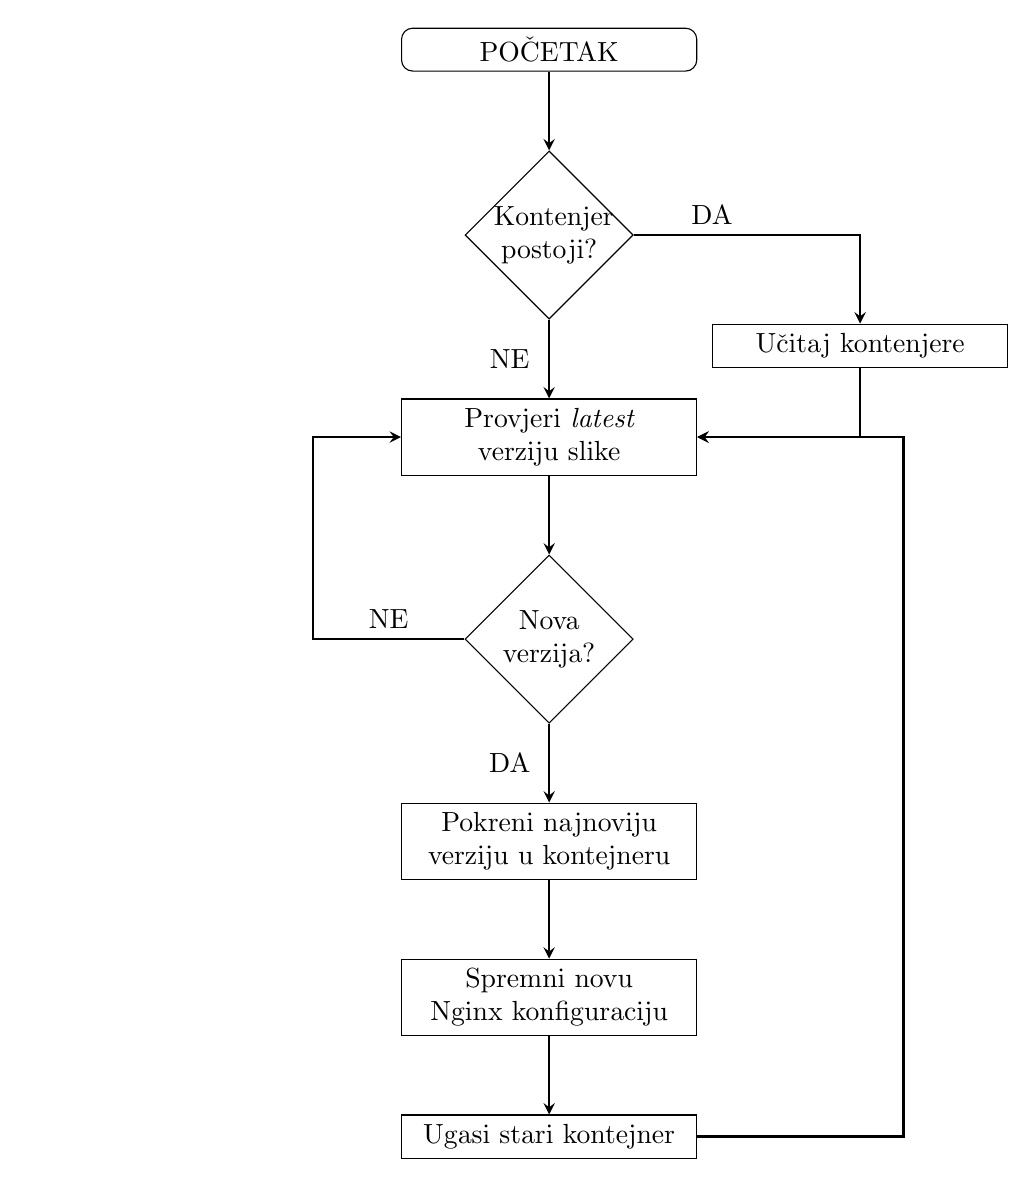
\begin{tikzpicture}[
        scale=1.0,
        node distance=1cm,
        text width=3.5cm,
        text centered,
        block/.style={
            rectangle,
            draw,
            text width=10em,
            text centered,
            rounded corners,
        },
        process/.style={
            rectangle,
            draw,
            text width=10em,
            text centered,
        },
        decision/.style={
            diamond,
            draw,
            text width=4em,
            text badly centered,
            inner sep=0pt,
        },
        arrow/.style={
            thick,->,>=stealth
        },
    ]
        \node [block] (start) {POČETAK};
        \node [decision, below=of start] (exists) {Kontenjer postoji?};

        \node [right=of exists] (e1) {};
        \node [process, below=of e1] (readstate) {Učitaj kontenjere};

        \node [process, below=of exists] (checkversion) {Provjeri \textit{latest} verziju slike};

        \node [left=of checkversion] (e2) {};

        \node [decision, below=of checkversion] (newversion) {Nova verzija?};

        \node [process, below=of newversion] (launch) {Pokreni najnoviju verziju u kontejneru};
        \node [process, below=of launch] (save) {Spremni novu Nginx konfiguraciju};
        \node [process, below=of save] (shutdown) {Ugasi stari kontejner};

        \draw [arrow] (start) -- (exists);
        \draw [arrow] (exists) -| node[anchor=south east] {DA} (readstate);
        \draw [arrow] (readstate) |- (checkversion);
        \draw [arrow] (exists) -- node[xshift=-5mm] {NE} (checkversion);
        \draw [arrow] (checkversion) -- (newversion);
        \draw [arrow] (newversion) -- node[anchor=south] {NE} ++(-3cm,0cm) |- (checkversion);

        \draw [arrow] (newversion) -- node[xshift=-5mm] {DA} (launch);
        \draw [arrow] (launch) -- (save);
        \draw [arrow] (save) -- (shutdown);
        \draw [arrow] (shutdown) -- ++(+4.5cm,0cm) |- (checkversion);
    \end{tikzpicture}
    \caption{Dijagram toka servisa za menadžment}%
    \label{fig:03servismanagement}
\end{figure}




\section{Razvoj nove verzije fibonacci aplikacije}
U drugoj verziji poboljšana je vremenska kompleksnost tako što je uklonjena rekurzija te dodana
memoizacija. Nova vremenska kompleksnost je $O(N)$, dok je memorijska kompleksnost $O(1)$. Nova
verzija prikazana je kodom~\ref{04fibv2}. U novoj je verziji također izmijenjen dizajn kao što je
prikazano slikom~\ref{fig:04redesign}

\lstset{caption={Fibonacci v2}, label=04fibv2}
\begin{lstlisting}[float=h]
func fibonacci(n uint64) uint64 {
	if n == 0 {
		return 0
	}
	a := uint64(0)
	b := uint64(1)

	for n > 1 {
		tmp := a + b
		a = b
		b = tmp
		n--
	}
	return b
}
\end{lstlisting}

\begin{figure}[h]
    \centering
    \includegraphics[width=0.5\textwidth]{img/04/new_app.png}
    \caption{Novi dizajn fibonacci aplikacije}%
    \label{fig:04redesign}
\end{figure}

Nakon što su napravljene izmjene unutar aplikacije, potrebno je spremiti izmjene unutar Git
repositorija te poslati izmjene na servis za pregled koda. Primjer za spremanje izmjena i slanje na
udaljeni Git poslužitelj pomoću komandne linije prikazan je kodom~\ref{04gitreview}.

\lstset{caption={Spremanje i slanje izmjena na Git poslužitelj}, label=04gitreview}
\begin{lstlisting}[float=h]
# nova git grana pod nazivom optimizacija
git checkout -b optimizacija

# dodaj datoteku main.go koja sadrzi izmjene
git add main.go

# dodaj izmjenu
git commit -m "Optimizacija fibonacci funkcije"

# posalji izmjene na server i prati udaljenu granu
git push -u origin optimizacija
\end{lstlisting}

Kada je kod pregledan i odobren tada se prebacuje u \textit{master} granu. Sustavi za reviziju koda
u pravilu to automatski odrađuju nakon što je kod potvrđen za spajanje. Ručno prebacivanje prikazano
je kodom~\ref{04gitmerge}.

\lstset{caption={Spremanje i slanje izmjena na Git poslužitelj}, label=04gitmerge}
\begin{lstlisting}[float=h]
# prelazak u master git granu
git checkout master

# spajanje grane optimizacija u granu master
git merge optimizacija

# posalji izmjene na server, master grana
git push origin master
\end{lstlisting}

Jenkins pokreće izgradnju nove aplikacije čim je nekakva izmjena dostupna na Git poslužitelju unutar
glavne, \textit{master} grane. Ukoliko su svi testovi uspješni objavljuje se Docker slika. Zatim
servis za menadžment dohvaća novu verziju te počinje posluživati korisnike s novom verzijom.

Prethodnu verziju aplikacije potrebno je ukloniti tek nakon što su svi zahtjevi obrađeni. Na
primjer, ukoliko je potrebno dvije sekunde za obradu nekog zahtjeva, tada je potrebno pričekati
barem toliko vremena prije nego što se prethodna verzija aplikacije može potpuno ugasiti.  U
protivnom zahtjev korisnika će biti prekinut i neće biti potpuno ispunjen.

Testiranje stabilnosti aplikacije prilikom izmjene koda provedeno je alatom \textit{Jmeter}. Jmeter
je alat za stresno testiranje aplikacije, a razvija ga neprofitna organizacija \textit{Apache}. Može
se koristiti za stresno testiranje FTP, LDAP, HTTP, baza podataka preko JDBC, i mnogih drugih
protokola.

Za testiranje infrastrukture ovog projekta korišten je HTTP protokol. Izvršeno je 10.000 zahtjeva
za 34.~fibonaccijev broj. U trenutku pokretanja stresnog testa korištena je stara verzija fibonacci
aplikacije, a potom je objavljena nova verzija koja sadrži optimizaciju. Svi zahtjevi uspješno su
izvršeni. Na slici~\ref{fig:04stresstest} prikazan je vremenski odaziv prve i druge verzije
aplikacije.

\begin{figure}[h]
    \centering
    \includegraphics[width=\textwidth]{img/04/response_time.png}
    \caption{Vrijeme odaziva aplikacije}%
    \label{fig:04stresstest}
\end{figure}

\section{Tipični problemi s objavom nove verzije aplikacije}
Bilo koja izmjena aplikacije može uzrokovati neočekivanu pogrešku, stoga svaka izmjena aplikacije
predstavlja rizik. Osim logičkih grešaka unutar aplikacije, koje se mogu otkriti testovima jedinice
i \textit{end-to-end} testovima, moguće se i greške koje se događaju samo prilikom objavljivanja
nove verzije. Primjerice, aplikacija može zapisivati podatke unutar baze podataka u određenom
formatu koji nije kompatibilan s novom verzijom aplikacije. Vraćanje na prethodnu verziju aplikacija
može dovesti i do dodatnih komplikacija ukoliko korisnik u trenutku ima novu verziju s novom bazom
podataka.

Tipični problemi s objavom nove verzije aplikacija su:
\begin{itemize}
    \item nekompatibilnost privremene memorije (\textit{engl. cache})
    \item nekompatibilnost baze podataka
    \item nekompatibilnost programskog sučelja klijenta i poslužitelja
\end{itemize}

Nekompatibilnost privremene memorije javlja se kada nova verzija aplikacije promjeni strukturu
privremene memorije te očita neočekivan podatak generiran iz prijašnje verzije aplikacije. Situacija
se može dodatno zakomplicirati ako su u danom trenutku pokrenute dvije verzije. Kako bi se izbjegla
takva situacija najčešće se preporuča novi ključ za privremenu memoriju ili progresivna izmjena
podataka privremene memorije. Prilikom korištenjem novog ključa nova aplikacija piše u novu
privremenu memoriju te ne ovisi o prethodnoj verziji. Ovakvo rješenje ima problem s hladnom
predmemorijom (\textit{engl. cold cache}) koje uzrokuje s povećanim vremenom odaziva. Druga opcija
je progresivna izmjena podataka koja zahtjeva dodatni kod kako bi stari i novi unos bio kompatibilan
s obje verzije aplikacije. Potrebne su barem dvije verzije i neko vrijeme kako bi se mogla ispustiti
podrška za prethodnu strukturu predmemorije.

Na primjeru fibonacci aplikacije, zamislimo da koristimo sustav za memoriju, kao na primjer
\textit{memcached}. U trenutnoj verziji aplikacija sprema vrijednost N-tog fibonaccijev broja pod
ključem \textit{fibonacci-N}. U trenutnoj verziji aplikacije odlučeno je da je prvi fibonaccijev
broj nula, a drugi broj jedan. No u novoj verziji aplikacije odlučeno je koristiti originalnu
verziju algoritma, tako da su i prvi i drugi fibonaccijevi brojevi jednaki broju jedan. Ukoliko se
rezultati memorije ne uklone ili spreme pod drugim ključem, tada će nova verzija fibonacci
aplikacije i dalje vraćati stare rezultate.

Nekompatibilnost baze podataka je slična nekompatibilnosti privremene memorije. No za razliku od
privremene memorije, nije moguće izabrati novi ključ jer u tom slučaju stari podaci neće biti
dostupni korisniku. Inženjer može izabrati migraciju sa stankom aplikacije ili bez stanke. Migracija
sa stankom aplikacije je u pravilu jednostavnija izvedba. No, takva stanka je negativno korisničko
iskustvo. Firme poput Google i Facebook uvijek koriste migracije bez stanke. Kako bi se migracija
mogla napraviti bez stanke potrebno je nekoliko faza i verzija aplikacija. Često se takva migracija
svodi na:
\begin{itemize}
    \item izmjene sheme baze podataka, ali takve izmjene da su kompatibilne sa prethodnom verzijom
        aplikacije
    \item izmjene aplikacije koja omogućava zapis u izmijenjenu bazu podataka bez da utječe na
        prethodnu verziju aplikacije
    \item prijepis povijesnih podataka u novu shemu (\textit{engl. backfill})
    \item izmjene aplikacije tako da se ne zapisuju podaci u staru shemu baze podataka
    \item izmjene sheme baze podataka gdje se stare vrijednosti uništavaju.
\end{itemize}

Kod nekompatibilnosti programskog sučelja klijenta i poslužitelja dolazi prilikom objave nove
aplikacije i promjenom sučelja na poslužitelju, to jest aplikaciji. Slika \ref{fig:04request_flow}
prikazuje pojednostavljeni primjer korisničke interakcije s fibonacci aplikacijom prilikom objave
nove verzije aplikacije.

\begin{figure}[h]
    \centering
    \includegraphics[width=\textwidth]{img/04/request_flow.png}
    \caption{Objava nove verzije aplikacije}%
    \label{fig:04request_flow}
\end{figure}

Korisnik prvo zahtjeva početnu HTML stranicu koja sadrži formu i klijentski Javascript kod koji
određuje gdje će se zahtjev poslati nakon što korisnik upiše broj i pritisne gumb "Računaj". Na
slici, prvi zahtjev je prema aplikacijskom sučelju (API) originalne verzije. No, drugi zahtjev
upućen je novoj verziji aplikacije. Ukoliko nova verzija ima drugačije sučelje, takav zahtjev neće
uspjeti te će korisniku biti poslana greška. Jedini način da web aplikacija ponovno proradi je tako
da korisnik ručno osvježi (\textit{engl. refresh}) web stranicu, što je negativno korisničko
iskustvo.

Kako bi se to izbjeglo, potrebno je zadržati kompatibilnost programskog sučelja trenutne i nove
verzije aplikacije. Nakon određenog vremena se može očekivati da će korisnici imati novu klijentsku
verziju aplikacije te se kompatibilnost može maknuti. U praksi se zna i pitati korisnika za
osvježavanje stranice.

\section{Vraćanje na staru aplikaciju}
Kao što je rečeno u prethodnom poglavlju, svaka izmjena aplikacije može uzrokovati s neočekivanom
pogreškom. Korištenjem testova jedinica i \textit{end-to-end} testova povećana je vjerojatnost
otkrivanja greške prilikom razvoja aplikacije. No, ukoliko novoobjavljena verzija aplikacije sadrži
neku grešku, potreban je dobar sustav kako bi se takva pogreška mogla brzo otkloniti. Često je
najbrže rješenje vraćanje na staru verziju aplikacije (\textit{engl.~version rollback}), gdje se
neispravna verzija zamjenjuje s prethodno objavljenom, stabilnom verzijom. Zatim je potrebno
ukloniti grešku u kodu te dodati prikladne testove nakon čega se može objaviti nova, ispravljena
verzija aplikacije.

Proces vraćanja na staru verziju mora biti brz i intuitivan. U ovom radu korišten je
parametrizitrani Jenkins posao za vraćanje na prethodno objavljenu verziju, prikazan
slikom~\ref{fig:04jenkins_rollback} i kodom~\ref{04:jenkins_revert}. Prilikom pokretanja takvog
posla korisniku je dan padajući izbornik sa svim verzijama aplikacije. Nakon što korisnik izabere
željenu verziju, Jenkins označava tu verziju aplikacije kao zadnju. Unutar trideset sekundi servis
za menadžment pokreće novoizabranu verziju aplikacije i počinje ju posluživati. U tom trenutku
verzija aplikacije s greškom se više ne poslužuje korisnicima.

\begin{figure}[h]
    \centering
    \includegraphics[width=\textwidth]{img/04/jenkins_rollback.png}
    \caption{Jenkins posao za vraćanje verzije aplikacije}%
    \label{fig:04jenkins_rollback}
\end{figure}

\lstset{caption={\textit{Jenkinsfile} za vraćanje na prethodnu verziju}, label=04:jenkins_revert}
\begin{lstlisting}[float=h]
pipeline {
    agent any
    stages {
        stage('Objava slike') {
            steps {
                script {
                    docker.withRegistry('https://docker.io', 'dockerhub') {
                        def i = docker.image("sokac/fibonacci:${VERZIJA_NUMBER}")
                        i.push('latest')
                    }
                }
            }
        }
    }
}
\end{lstlisting}


\chapter{Zaključak}
Zaključak TODO

\bibliography{literatura}
\bibliographystyle{ferit}

\begin{sazetak}
Sažetak na hrvatskom jeziku.
\kljucnerijeci{Ključne riječi, odvojene zarezima.}
\end{sazetak}

\engtitle{Continuous deployment}
\begin{abstract}
Abstract.

\keywords{Keywords, comma separated.}
\end{abstract}

\end{document}
